
\section{Constant Subcritical flow}

This is a very simple test of constant (subcritical) flow down a channel. The constant state should be preserved. 


\subsection{Results}
For our test we consider the initial condition
\begin{equation}
u(x,y,0)=v(x,y,0)=0\,, \quad
w(x,y,0)= 1.5\,,
\end{equation}
and the Dirichlet boundary conditions at $x=0^{-}$ and $25^{+}$ to be 
\begin{equation}
[w,hu,hv]=[2, 4.42, 0]\,.
\end{equation}
Representatives of the simulation results are given in the following three figures. 
We should see a very accurate reproduction of the steady flow $w=2$ $u=2.21$, $q=4.42$ by 50secs. 

\begin{figure}
\begin{center}
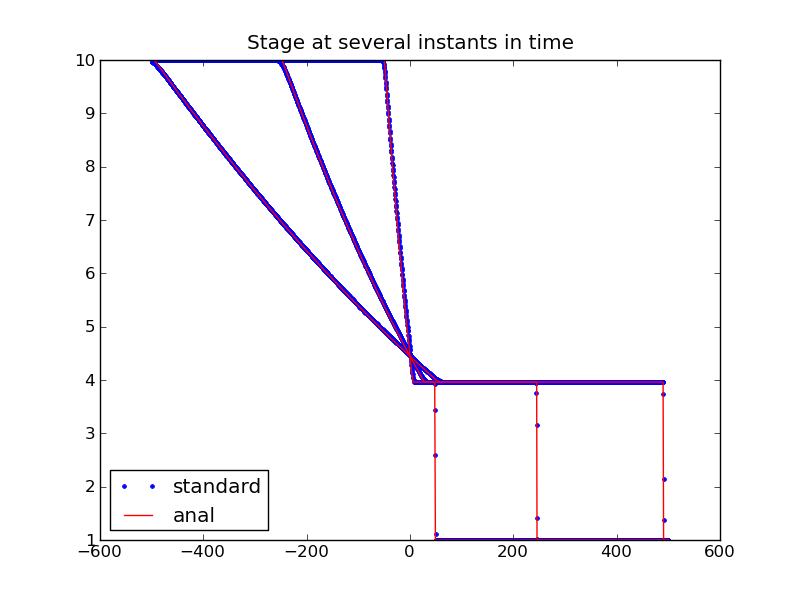
\includegraphics[width=0.9\textwidth]{stage_plot.png}
\end{center}
\caption{Stage results}
\end{figure}


\begin{figure}
\begin{center}
\includegraphics[width=0.9\textwidth]{xmom_plot.png}
\end{center}
\caption{Xmomentum results}
\end{figure}


\begin{figure}
\begin{center}
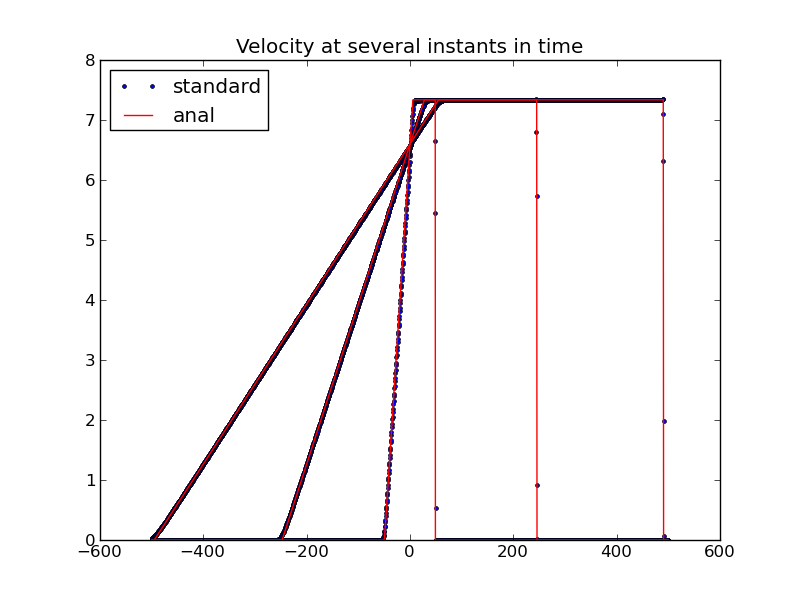
\includegraphics[width=0.9\textwidth]{xvel_plot.png}
\end{center}
\caption{Xvelocity results}
\end{figure}


\endinput
